\section{Conclusiones} 

En esta práctica, se implementó un convertidor digital-analógico (DAC) utilizando un muestreo controlado por un retardo en lugar de un temporizador. Esto permitió observar cómo se generaban diferentes frecuencias de salida a partir de valores digitales, lo que es fundamental en aplicaciones de procesamiento de señales. Al utilizar un retardo para el muestreo, se pudo observar cómo la frecuencia de salida variaba en función del tiempo de espera entre cada muestreo. Esto es crucial para entender cómo se puede manipular la señal de salida en un DAC. La implementación de la comunicación serial permitió cambiar dinámicamente la frecuencia de salida del DAC. Aprendí a utilizar el teclado para enviar comandos que modifican los parámetros de la señal, lo que demuestra la importancia de la interacción entre el usuario y el sistema. La comunicación serial es esencial en sistemas embebidos, ya que permite la configuración y el monitoreo en tiempo real de los dispositivos. Las imágenes del osciloscopio muestran diferentes formas de onda generadas por el DAC. A medida que se ajustaba la frecuencia, se podía observar cómo la forma de la señal cambiaba, lo que es indicativo de la calidad del muestreo y la resolución del DAC. Las variaciones en la frecuencia de muestreo también se reflejan en la forma de la señal, lo que resalta la importancia de un muestreo adecuado para obtener una representación precisa de la señal analógica. 

\begin{figure}[H]
      \centering
      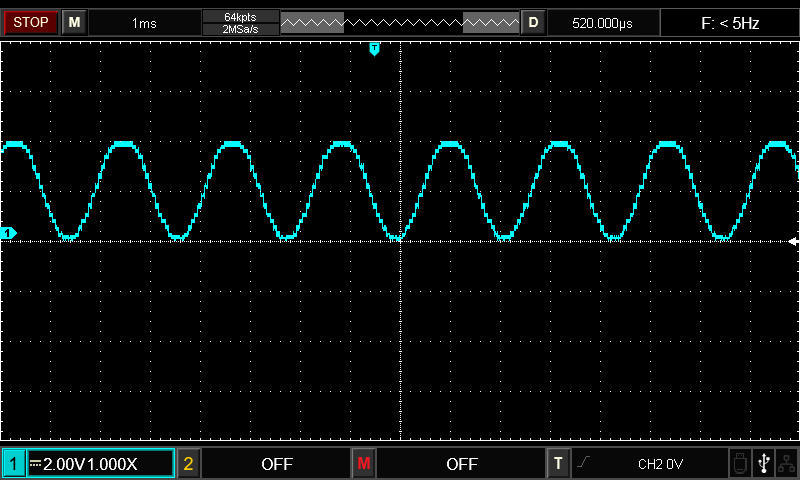
\includegraphics[width=0.5\textwidth]{images/500HZ}
      \captionof{figure}{Señal de $500\si{\Hz}$}
\end{figure}

\begin{figure}[H]
      \centering
      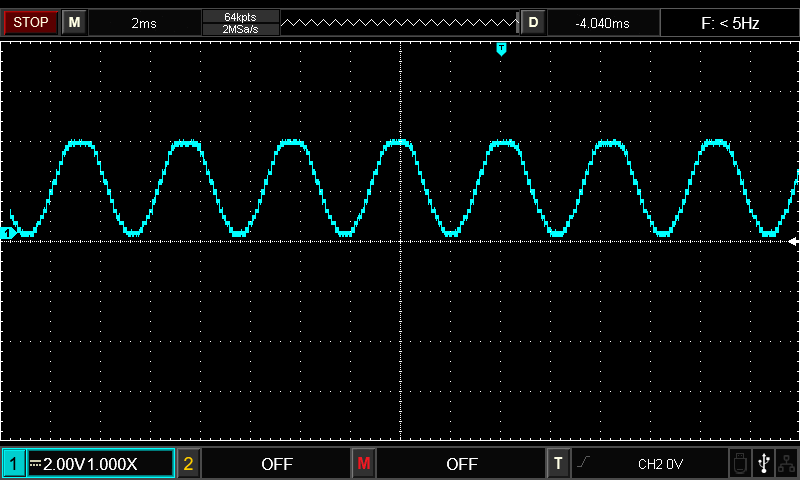
\includegraphics[width=0.5\textwidth]{images/250HZ}
      \captionof{figure}{Señal de $250\si{\Hz}$}
\end{figure}

\begin{figure}[H]
      \centering
      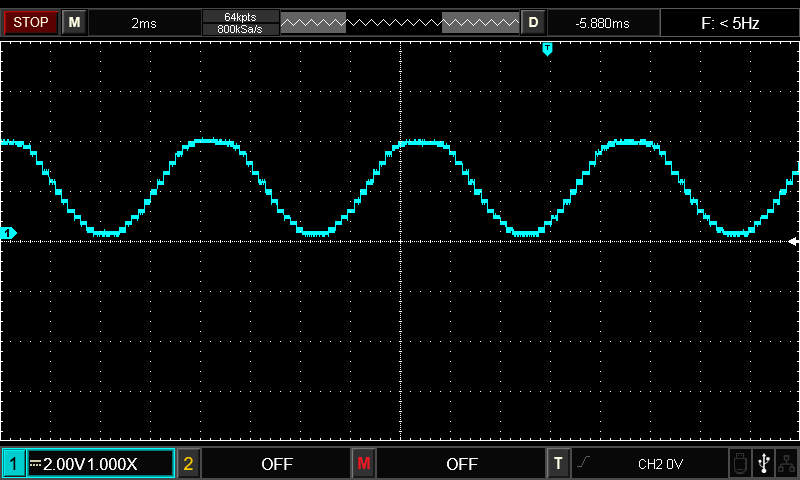
\includegraphics[width=0.5\textwidth]{images/125HZ}
      \captionof{figure}{Señal de $125\si{\Hz}$}
\end{figure}